\chapter{Proposed Method: DCOACH + Human Model}
\label{chapter:Proposed Method}

\section{Objective: Off-policy D-COACH}
\label{section:Objective: Off-policy D-COACH}


In order to truly leverage the advantages of experience replay it is necessary  to develop a novel off-policy D-COACH algorithm. To do so, it is proposed to incorporate a model that learns to predict the teacher’s feedback and include it in the D-COACH framework. This new model, that we call the Human Model and which is represented by a neural network, should learn which feedback is required for a given state/action pair. The Human Model will be updated with batches of states and actions stored in a replay buffer. Then, the model will output a batch of feedback predictions that, together with the correspondent batch of feedback provided by the human from the buffer, will update the Human Model's weights via supervised learning, see figure \ref{fig:update_human_model}. 


\begin{figure}[H]
    \centering
    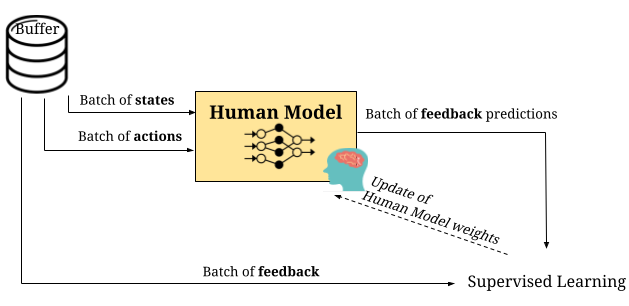
\includegraphics[width=.7\textwidth]{figures/train_human_model.png}
    \caption{Update of the Human Model}
    \label{fig:update_human_model}
\end{figure}


\section{The Human Model}
\label{section:The Human Model}


Figure \ref{fig:update_agent} depicts how the agent's policy will be updated with off-policy corrections indirectly through the Human Model. The Human Model will be able to provide feedback to the newest version of the agent’s policy from a batch of states sampled from the replay buffer. This batch of states will be pass to both the agent's policy and the human model. Then, the agent's policy will output a batch of actions that will be fed to the human model. This batch of actions together with the output of the Human Model, will serve to update the weights of the agent's policy. Both models, the agent and the human ones could be learned in parallel.




\begin{figure}[H]
    \centering
    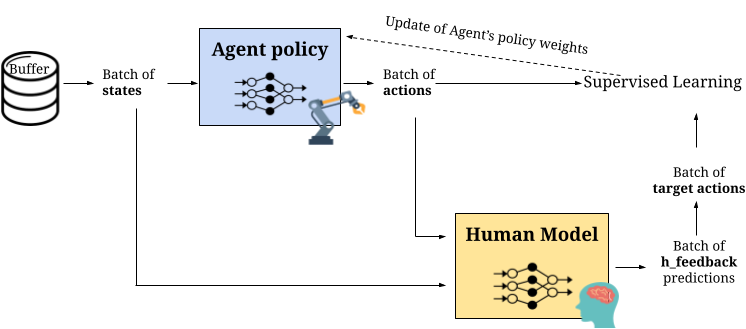
\includegraphics[width=.8\textwidth]{figures/train_agent.png}
    \caption{Update of the agent's policy}
    \label{fig:update_agent}
\end{figure}



\begin{figure}[H]
\centering
\usetikzlibrary{positioning, fit, calc}   
  
\tikzset{block/.style={draw, thick, text width=2.5cm ,minimum height=1.1cm, align=center},   
line/.style={-latex}     
}  
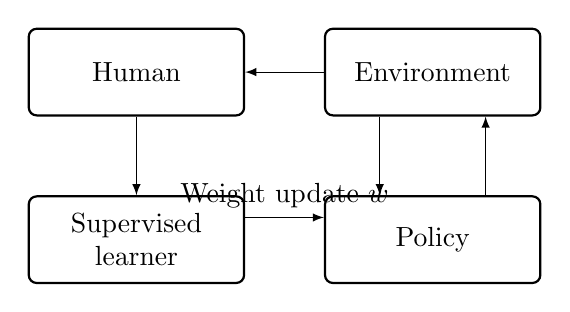
\begin{tikzpicture}  
\node[block, rounded corners=0.1cm] (human) {Human};  
\node[block,right=of human, rounded corners=0.1cm] (env) {Environment};   
\node[block, below=of env, rounded corners=0.1cm] (policy) {Policy}; 

\node[block, below=of human, rounded corners=0.1cm] (sup) {Supervised learner};  

 \draw[line] (env)-- (human);  
 %\draw[line] (policy)-- (env);  
% \draw[line] (env)-- (policy);  
 %\draw[->] (policy.140) -- (env.220);
 %\draw[->] (env.60) -- (policy.300);
 
 %\draw[red, very thick] (env.80)-- ++(1.3cm,1.3cm);
 \draw[line](env.220) -- (policy.140);
\draw[line](policy.40) -- (env.320);
\draw[line] ($(sup.north east)!0.25!(sup.south east)$) -- node[above] {Weight update $w$} ($(policy.north west)!0.25!(policy.south west)$);
 \draw[line](human.south) -- (sup.north);
    
\end{tikzpicture}  
\caption{Autoencoder, \cite{Autoencoder-tikz}} \label{fig:autoencoder}
\end{figure}



\begin{figure}[H]
\centering
\begin{tikzpicture}
  [block/.style={draw,minimum width=#1,minimum height=2em},
  block/.default=10em,high/.style={minimum height=3em},auto,
  node distance=5mm]
  %node distance=5em,auto]
  % Nodes
  \node[block=3cm,high] (n0) {Input};
  \node[block=3cm,high,right=1cm of n0] (env) {Environment};
  \node[block=3cm,high,below=of env] (policy) {Policy};
  \node[block=3cm,high,right=of policy] (PSL) {Policy Supervise Learner};
  \node[block=3cm,high,right=of policy] (HM) {Human Model};
  \node[right=1cm of PSL,align=center] (n4) {Measurement\\File};
  
  
  \draw[double,double distance=3pt,{<[policy]}-{>[US]},bend left](A)to(B){};
  \draw[double,double distance=3pt,{<[UK]}-{>[UK]},bend left](B)to(A){};

\end{tikzpicture}
\caption{Autoencoder, \cite{Autoencoder-tikz}} \label{fig:autoencoder}
\end{figure}

\section{Complete algorithm}
\label{section:Complete algorithm}


\begin{algorithm}[H]
\caption{Deep COACH + HM}\label{algorithm:DeepCOACH}
\begin{algorithmic}[1]
\State \textbf{Require:} error magnitude $e$, buffer update interval $b$
\State \textbf{Init:} $\mathcal{D} = [\quad]$  \emph{\# initialize memory buffer}
\For{t = 1,2,...}{}
\State \textbf{observe} state $o_{t}$
\State \textbf{execute} action $a_{t}=\pi_{\theta}(o_{t})$
\State \textbf{feedback} human corrective advice $h_{t}$
\If{$h_{t}$ is not \textbf{0}}
\State \textbf{append} $(o_{t}, a_{t}, h_{t})$ to $\mathcal{D}$
\State $\mathit{error}_{t} = h_{t}\cdot e$
\State $a_{target(t)} = a_{t} + \mathit{error}_{t}$
\State \textbf{update} $\pi_\theta$ using SGD with pair ($o_{t}$, $a^{\text{target}}_{t}$)
\State \textbf{update} $\text{HumanModel}_\omega$ using SGD with a mini-batch sampled from $\mathcal{D}$
\State  $a=\pi_{\theta}(o)$ \emph{\# where $o$ is a batch of observations sampled from $\mathcal{D}$}
\State  $\hat{h}=\text{HumanModel}_\omega(a, o)$
\State \textbf{update} $\pi_\theta$ using SGD with batch $a$ and batch $\hat{h}$
\EndIf
\If{mod(t, b) is 0 }
\State \textbf{update} $\text{HumanModel}_\omega$ using SGD with a mini-batch sampled from $\mathcal{D}$
\State  $a=\pi_{\theta}(o)$ \emph{\# where $o$ is a batch of observations sampled from $\mathcal{D}$}
\State  $\hat{h}=\text{HumanModel}_\omega(a, o)$
\State \textbf{update} $\pi_{\theta}$ using SGD with batch $a$ and batch $\hat{h}$
\EndIf
\EndFor
\end{algorithmic}
\label{al:D-COACH with HM}
\end{algorithm}


\section{Discussion}
\label{section:Algorithm-Discussion}
Tell about the problem that at the beginning, the Human Model is not learnt yet and can be a drawback and that is why we put a smaller learning rate